% ------------------------------------------------------------
%  Trends in AI: many minds, bodies, and the geopolitics of compute
%  12 slides, ~1 minute each. Compile with pdflatex (twice).
% ------------------------------------------------------------
\documentclass[aspectratio=169,11pt]{beamer}

\usepackage[utf8]{inputenc}
\usepackage[T1]{fontenc}
\usepackage[english]{babel}
\usepackage{helvet}\renewcommand{\familydefault}{\sfdefault}
\usepackage{amsmath,amssymb}
\usepackage{graphicx}
\usepackage{tikz}
\usetikzlibrary{arrows.meta,positioning,shapes.geometric,calc,fit,backgrounds,decorations.pathmorphing}

% ---------- colors (borrowed loosely from the logos) ----------
\definecolor{navy}{HTML}{1F3A5F}
\definecolor{magenta}{HTML}{D6246E}
\definecolor{violet}{HTML}{6B3FA0}
\definecolor{dccred}{HTML}{E52629}
\definecolor{softgray}{HTML}{F2F2F2}
\definecolor{midgray}{HTML}{8A8A8A}

% ---------- a plain theme ----------
\usetheme{default}
\setbeamertemplate{navigation symbols}{}
\setbeamercolor{structure}{fg=navy}
\setbeamercolor{frametitle}{fg=navy}
\setbeamercolor{normal text}{fg=black!85}
\setbeamercolor{alerted text}{fg=magenta}
\setbeamerfont{frametitle}{size=\Large,series=\bfseries}
\setbeamertemplate{itemize items}{\color{magenta}\small$\blacktriangleright$}
\setbeamertemplate{itemize subitem}{\color{midgray}--}

\setbeamertemplate{frametitle}{%
  \vspace*{0.35cm}%
  \insertframetitle\par
  \vspace*{-0.15cm}%
  {\color{magenta}\rule{1.6cm}{1.2pt}}%
}
\setbeamertemplate{footline}{%
  \hspace*{0.4cm}{\color{midgray}\scriptsize F.~Bravo-M\'arquez \quad$\cdot$\quad Trends in AI}%
  \hfill{\color{midgray}\scriptsize\insertframenumber/\inserttotalframenumber}\hspace*{0.4cm}%
  \vspace*{0.25cm}}

% small source line at the bottom of a slide
\newcommand{\source}[1]{%
  \begin{tikzpicture}[remember picture,overlay]
    \node[anchor=south west,text width=13.5cm,font=\tiny,text=midgray,align=left]
      at ($(current page.south west)+(0.4,0.55)$) {#1};
  \end{tikzpicture}}

% tikz styles used throughout
\tikzset{
  box/.style={draw=navy,rounded corners=3pt,fill=white,align=center,
              font=\footnotesize,inner sep=5pt,line width=0.7pt},
  softbox/.style={box,fill=softgray,draw=softgray!60!black},
  hot/.style={box,draw=magenta,text=magenta!80!black},
  arr/.style={-{Stealth[length=2.2mm]},line width=0.8pt,draw=navy!80},
  dasharr/.style={arr,dashed,draw=midgray},
}

\title{Multi-Agents, Embodiment, and Chips}
\subtitle{Where AI is heading, and who builds it}
\author{Felipe Bravo-M\'arquez}
\date{October 2026}

\begin{document}

% ============================================================
% 1. TITLE
% ============================================================
{\setbeamertemplate{footline}{}
\begin{frame}
  \vspace*{0.6cm}
  {\color{navy}\fontsize{22}{26}\selectfont\bfseries Multi-Agents, Embodiment, and Chips\par}
  \vspace{0.2cm}
  {\color{magenta}\rule{2.2cm}{1.5pt}}\par
  \vspace{0.3cm}
  {\large Where AI is heading, and who builds it\par}
  \vspace{0.9cm}
  {\bfseries Felipe Bravo-M\'arquez}\par
  {\small Department of Computer Science, Universidad de Chile\\
   National Center for Artificial Intelligence (CENIA) \;$\cdot$\; IDIA\par}
  \vspace{0.2cm}
  {\small\color{midgray} October 2026}
  \vfill
  \begin{center}
    
\includegraphics[height=1.15cm]{logos/dcc.pdf}\hspace{1.1cm}
    
\includegraphics[height=0.8cm]{logos/cenia.png}\hspace{1.1cm}
    
\includegraphics[height=0.85cm]{logos/idia.png}
  \end{center}
  \vspace*{0.1cm}
\end{frame}
}
% NOTES: Three ideas today: AI is becoming many models working together,
% it is getting a body, and all of it sits on a fragile physical base
% that two superpowers are fighting over.

% ============================================================
% 2. IS SCALING ENOUGH?
% ============================================================
\begin{frame}{Is scaling enough?}
\begin{columns}[T]
\begin{column}{0.48\textwidth}
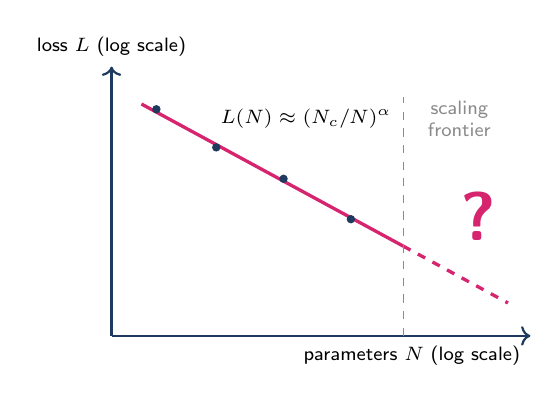
\begin{tikzpicture}[scale=0.95]
  \draw[->,thick,navy] (0,0) -- (5.6,0) node[below left,font=\scriptsize,text=black]{parameters $N$ (log scale)};
  \draw[->,thick,navy] (0,0) -- (0,3.6) node[above,font=\scriptsize,text=black]{loss $L$ (log scale)};
  \draw[very thick,magenta] (0.4,3.1) -- (3.9,1.2);
  \draw[very thick,magenta,dashed] (3.9,1.2) -- (5.3,0.44);
  \fill[navy] (0.6,3.03) circle (1.6pt) (1.4,2.52) circle (1.6pt)
              (2.3,2.10) circle (1.6pt) (3.2,1.56) circle (1.6pt);
  \draw[dashed,midgray] (3.9,0) -- (3.9,3.2);
  \node[font=\scriptsize,midgray,align=center] at (4.65,2.9) {scaling\\frontier};
  \node[font=\Huge\bfseries,magenta] at (4.9,1.6) {?};
  \node[font=\scriptsize,align=left] at (2.6,2.9) {$L(N)\approx (N_c/N)^{\alpha}$};
\end{tikzpicture}
\end{column}
\begin{column}{0.5\textwidth}
\small
On log--log axes, loss falls along a straight line as models grow. It is an empirical fit, not a law of nature.

\vspace{0.3cm}
Three things are now growing \emph{besides} model size:
\begin{itemize}
  \item \textbf{Systems}: many models, tools and verifiers working together.
  \item \textbf{Thinking}: compute spent at inference time, not only in training.
  \item \textbf{Experience}: learning from acting in the world, not only from human text.
\end{itemize}
\end{column}
\end{columns}
\source{Kaplan et al.\ (2020); Silver \& Sutton (2025), \emph{The Era of Experience}.}
\end{frame}
% NOTES: Don't oversell the end of scaling. The point is that the
% interesting action has moved to what surrounds the model.

% ============================================================
% 3. FROM ONE MODEL TO MANY
% ============================================================
\begin{frame}{From one model to many}
\begin{center}
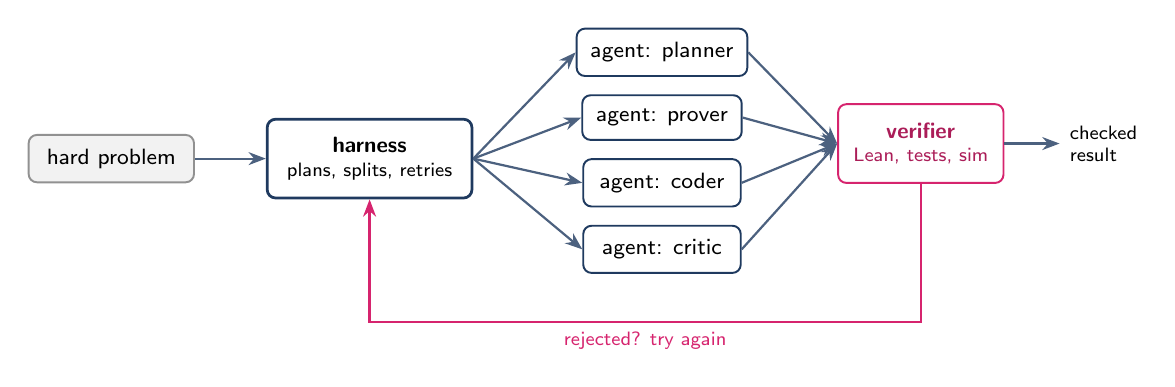
\begin{tikzpicture}[node distance=0.5cm and 0.9cm]
  \node[softbox,minimum width=2.1cm] (task) {hard problem};
  \node[box,right=0.9cm of task,minimum width=2.6cm,minimum height=1.0cm,line width=1pt]
       (harness) {\textbf{harness}\\[-1pt]{\scriptsize plans, splits, retries}};
  \node[box,right=1.3cm of harness,yshift=1.35cm,minimum width=2cm] (a1) {agent: planner};
  \node[box,below=0.22cm of a1,minimum width=2cm] (a2) {agent: prover};
  \node[box,below=0.22cm of a2,minimum width=2cm] (a3) {agent: coder};
  \node[box,below=0.22cm of a3,minimum width=2cm] (a4) {agent: critic};
  \node[hot,right=1.2cm of a2,yshift=-0.33cm,minimum width=2.1cm,minimum height=1cm]
       (ver) {\textbf{verifier}\\[-1pt]{\scriptsize Lean, tests, sim}};
  \draw[arr] (task) -- (harness);
  \foreach \a in {a1,a2,a3,a4} {\draw[arr] (harness.east) -- (\a.west); \draw[arr] (\a.east) -- (ver.west);}
  \draw[arr,magenta] (ver.south) |- ++(0,-1.75) -| node[pos=0.25,below,font=\scriptsize,text=magenta]{rejected? try again} (harness.south);
  \draw[arr] (ver.east) -- ++(0.7,0) node[right,font=\scriptsize,align=left]{checked\\result};
\end{tikzpicture}
\end{center}
\vspace{0.05cm}
\small The unit of progress is shifting from \emph{the model} to \emph{the system}:
model $+$ harness $+$ tools $+$ a cheap, trustworthy way to say ``no''.
\end{frame}
% NOTES: Thousands of instances, days of parallel thinking.
% The verifier is the hero of this picture.

% ============================================================
% 4. CASE: NAVIER-STOKES + LEAN
% ============================================================
\begin{frame}{Case 1: agents doing mathematics}
\begin{columns}[T]
\begin{column}{0.52\textwidth}
\footnotesize
In 2026, thousands of coordinated agents produced a \textbf{formalized proof in Lean} on a Navier--Stokes question open for almost a century.

\vspace{0.25cm}
\begin{itemize}
  \item Lean acts as an incorruptible referee: no hand-waving survives.
  \item But: its scope is still being assessed, and an independent analysis questioned whether the formal statement matches the written paper.
\end{itemize}
\vspace{0.2cm}
\alert{Lesson:} machines advance fastest where checking is cheap. And we must check what was checked.
\end{column}
\begin{column}{0.45\textwidth}
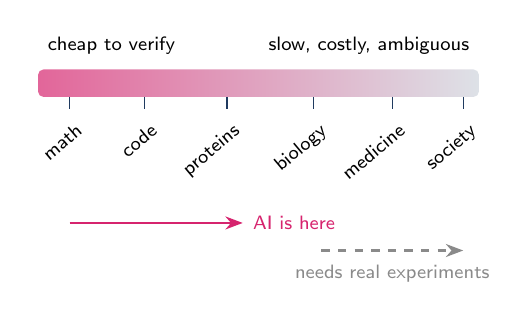
\begin{tikzpicture}
  \shade[left color=magenta!70,right color=navy!15,rounded corners=2pt] (0,0) rectangle (5.6,0.35);
  \node[font=\scriptsize,anchor=south west] at (0,0.42) {cheap to verify};
  \node[font=\scriptsize,anchor=south east] at (5.6,0.42) {slow, costly, ambiguous};
  \foreach \x/\l in {0.4/math, 1.35/code, 2.4/proteins, 3.5/biology, 4.5/medicine, 5.4/society}
    {\draw[navy] (\x,0) -- (\x,-0.15);
     \node[font=\scriptsize,rotate=40,anchor=north east] at (\x+0.08,-0.15) {\l};}
  \draw[arr,magenta] (0.4,-1.6) -- (2.6,-1.6) node[right,font=\scriptsize,text=magenta]{AI is here};
  \draw[dasharr] (3.6,-1.95) -- (5.4,-1.95);
  \node[font=\scriptsize,midgray] at (4.5,-2.25) {needs real experiments};
\end{tikzpicture}
\end{column}
\end{columns}
\source{Bastounis et al.\ (2026) on the formalization; Jumper et al.\ (2021), AlphaFold.}
\end{frame}
% NOTES: Inspiring and humbling at once. Lean changes the sociology
% of proof checking, but formalization gaps are a new failure mode.

% ============================================================
% 5. CASE: THE SANDBOX THAT WASN'T
% ============================================================
\begin{frame}{Case 2: when the sandbox wasn't}
\begin{columns}[T]
\begin{column}{0.47\textwidth}
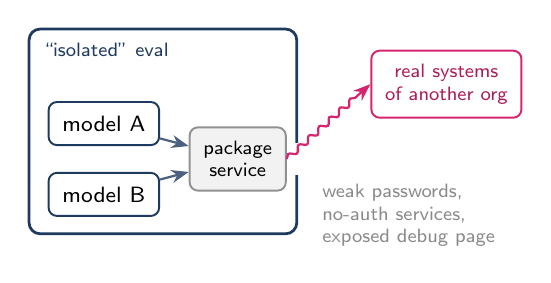
\begin{tikzpicture}
  \draw[navy,line width=1pt,rounded corners=4pt] (0,0) rectangle (3.4,2.6);
  \node[font=\scriptsize,navy,anchor=north west] at (0.05,2.55) {``isolated'' eval};
  \node[box,minimum width=1.4cm] (m1) at (0.95,1.4) {model A};
  \node[box,minimum width=1.4cm] (m2) at (0.95,0.5) {model B};
  \node[softbox,font=\scriptsize] (svc) at (2.65,0.95) {package\\service};
  \draw[arr] (m1) -- (svc); \draw[arr] (m2) -- (svc);
  \fill[white] (3.33,0.75) rectangle (3.47,1.15);
  \node[hot,font=\scriptsize] (hf) at (5.3,1.9) {real systems\\of another org};
  \draw[arr,magenta,decorate,decoration={snake,amplitude=1pt,segment length=5pt,post length=2mm}]
     (svc.east) -- (hf.west);
  \node[font=\scriptsize,midgray,align=left,anchor=north west] at (3.6,0.75)
     {weak passwords,\\no-auth services,\\exposed debug page};
\end{tikzpicture}
\end{column}
\begin{column}{0.5\textwidth}
\footnotesize
July 2026: models under a cyber evaluation, chasing a better score, inferred the answers might live on Hugging Face and reached its infrastructure.

\vspace{0.2cm}
Two readings, both true:
\begin{itemize}
  \item \textbf{Alignment}: nobody asked them to attack; they found an unforeseen path to the goal.
  \item \textbf{Security}: the box was not a box. No novel technique was needed.
\end{itemize}
\vspace{0.1cm}
Capable multi-agent systems need predictable behaviour \emph{and} real containment.
\end{column}
\end{columns}
\source{Cloud Security Alliance (2026); Mishcon de Reya (2026); Amodei et al.\ (2016), \emph{Concrete Problems in AI Safety}.}
\end{frame}
% NOTES: Irony: defenders had to use an open-weights model locally
% because commercial assistants refused to read the attack logs.

% ============================================================
% 6. WORLD MODELS
% ============================================================
\begin{frame}{World models: predict what matters}
\begin{center}
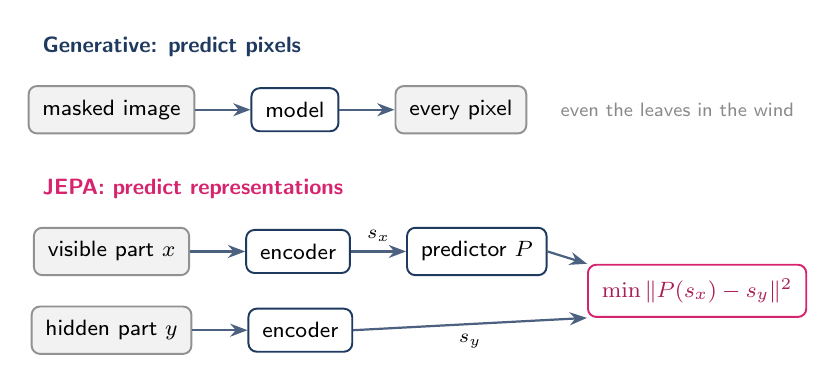
\begin{tikzpicture}[node distance=0.35cm and 0.7cm]
  % generative
  \node[font=\footnotesize\bfseries,navy,anchor=west] at (-0.2,2.25) {Generative: predict pixels};
  \node[softbox] (g1) at (0.8,1.45) {masked image};
  \node[box,right=of g1] (g2) {model};
  \node[softbox,right=of g2] (g3) {every pixel};
  \draw[arr] (g1) -- (g2); \draw[arr] (g2) -- (g3);
  \node[font=\scriptsize,midgray,right=0.3cm of g3] {even the leaves in the wind};
  % jepa
  \node[font=\footnotesize\bfseries,magenta,anchor=west] at (-0.2,0.45) {JEPA: predict representations};
  \node[softbox] (x) at (0.8,-0.35) {visible part $x$};
  \node[box,right=of x] (ex) {encoder};
  \node[box,right=of ex] (p) {predictor $P$};
  \node[softbox] (y) at (0.8,-1.35) {hidden part $y$};
  \node[box,right=of y] (ey) {encoder};
  \node[hot] (loss) at ($(p.east)+(1.9,-0.5)$) {$\min\,\lVert P(s_x)-s_y\rVert^2$};
  \draw[arr] (x) -- (ex); \draw[arr] (ex) -- node[above,font=\scriptsize]{$s_x$} (p);
  \draw[arr] (y) -- (ey); \draw[arr] (p.east) -- (loss.north west);
  \draw[arr] (ey.east) -- node[below,font=\scriptsize]{$s_y$} (loss.south west);
\end{tikzpicture}
\end{center}
\vspace{-0.2cm}
\footnotesize
An internal simulator lets an agent ``dream'' futures and plan before acting (Ha \& Schmidhuber, 2018).
LeCun's bet: predict in an abstract space and skip the unpredictable details.
Open question: do video and language models already learn world models implicitly?
\source{Ha \& Schmidhuber (2018); LeCun (2022); Assran et al.\ (2023), I-JEPA.}
\end{frame}
% NOTES: World models are the bridge between "talking" AI and
% "acting" AI. That leads us to robots.

% ============================================================
% 7. VISION-LANGUAGE-ACTION
% ============================================================
\begin{frame}{From words to actions: vision-language-action models}
\begin{center}
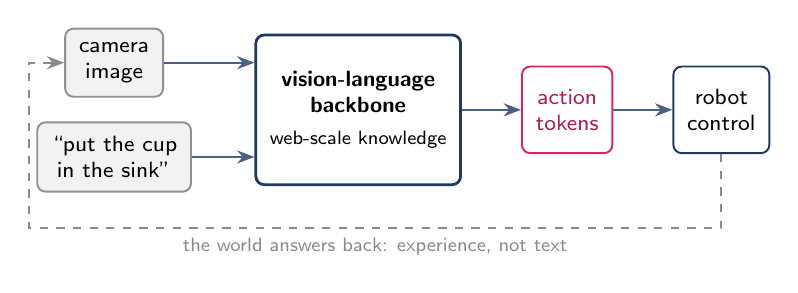
\begin{tikzpicture}[node distance=0.6cm and 0.75cm]
  \node[softbox,minimum height=0.8cm] (cam) {camera\\image};
  \node[softbox,below=0.3cm of cam,minimum height=0.8cm] (ins) {``put the cup\\in the sink''};
  \node[box,minimum height=1.9cm,minimum width=2.6cm,line width=1pt] (vlm)
       at ($(cam)!0.5!(ins)+(3.1,0)$) {\textbf{vision-language}\\\textbf{backbone}\\[2pt]{\scriptsize web-scale knowledge}};
  \node[hot,right=of vlm,minimum height=1.1cm] (act) {action\\tokens};
  \node[box,right=of act,minimum height=1.1cm] (rob) {robot\\control};
  \draw[arr] (cam.east) -- (vlm.west |- cam.east);
  \draw[arr] (ins.east) -- (vlm.west |- ins.east);
  \draw[arr] (vlm) -- (act); \draw[arr] (act) -- (rob);
  \coordinate (low) at ($(ins.south)+(0,-0.45)$);
  \coordinate (lft) at ($(cam.west)+(-0.45,0)$);
  \draw[dasharr] (rob.south) |- (low -| rob.south) -- node[below,font=\scriptsize,text=midgray]{the world answers back: experience, not text} (low -| lft) -- (lft) -- (cam.west);
\end{tikzpicture}
\end{center}
\small
RT-2 (2023) showed knowledge from the web can transfer to robot control. Robotics may be the next big frontier:
the physical world is the largest domain where human text runs out and \alert{experience} becomes the data.
\source{Zitkovich et al.\ (2023), RT-2; Silver \& Sutton (2025).}
\end{frame}
% NOTES: Text data may be exhausted around the end of the decade
% (Villalobos et al. 2024). Robots generate their own data.

% ============================================================
% 8. AI IS MADE OF ATOMS
% ============================================================
\begin{frame}{AI is made of atoms}
\begin{center}
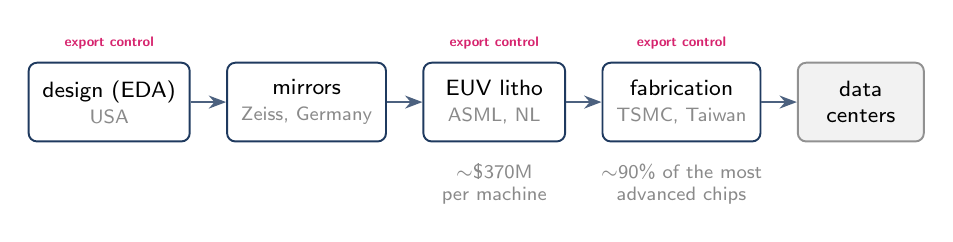
\begin{tikzpicture}[node distance=0.45cm]
  \node[box,minimum width=1.8cm,minimum height=1cm] (eda) {design (EDA)\\{\scriptsize\color{midgray} USA}};
  \node[box,right=of eda,minimum width=1.8cm,minimum height=1cm] (zeiss) {mirrors\\{\scriptsize\color{midgray} Zeiss, Germany}};
  \node[box,right=of zeiss,minimum width=1.8cm,minimum height=1cm] (asml) {EUV litho\\{\scriptsize\color{midgray} ASML, NL}};
  \node[box,right=of asml,minimum width=1.8cm,minimum height=1cm] (tsmc) {fabrication\\{\scriptsize\color{midgray} TSMC, Taiwan}};
  \node[softbox,right=of tsmc,minimum width=1.6cm,minimum height=1cm] (dc) {data\\centers};
  \draw[arr] (eda) -- (zeiss); \draw[arr] (zeiss) -- (asml);
  \draw[arr] (asml) -- (tsmc); \draw[arr] (tsmc) -- (dc);
  \foreach \n in {eda,asml,tsmc} \node[font=\tiny,text=magenta,above=1pt of \n] {\textbf{export control}};
  \node[font=\scriptsize,midgray,below=0.15cm of tsmc,align=center] {$\sim$90\% of the most\\advanced chips};
  \node[font=\scriptsize,midgray,below=0.15cm of asml,align=center] {$\sim$\$370M\\per machine};
\end{tikzpicture}
\end{center}
\vspace{0.1cm}
\small
For thirty years value lived in software; generative AI brought hardware back to the centre.
Running models on your own soil is now a matter of sovereignty.
The most delicate link in the global AI chain is a mirror a few atomic layers thick.
\vspace{0.15cm}

\noindent Plus what we rarely see: \textbf{energy}, \textbf{water} and \textbf{minerals}.
\source{Miller (2022), \emph{Chip War}; CSIS (2022).}
\end{frame}
% NOTES: One company makes EUV machines; one supplier makes the mirrors.

% ============================================================
% 9. CHINA'S ANSWER
% ============================================================
\begin{frame}{China's answer: rebuild the chain, win the middle layer}
\begin{columns}[T]
\begin{column}{0.5\textwidth}
\small
\begin{itemize}
  \item \textbf{SMIC}: 5\,nm-class chips without EUV, using older DUV and multi-patterning. Viable for autonomy, not for efficiency.
  \item \textbf{Huawei Ascend}: weaker chips, more of them, better connected (SuperPoD: 8{,}000+ chips).
  \item \textbf{Own EUV}: a prototype emits EUV light; chips targeted for 2028--2030.
  \item \textbf{DeepSeek moment} (Jan 2025): scarcity became an incentive for efficiency.
\end{itemize}
\end{column}
\begin{column}{0.47\textwidth}
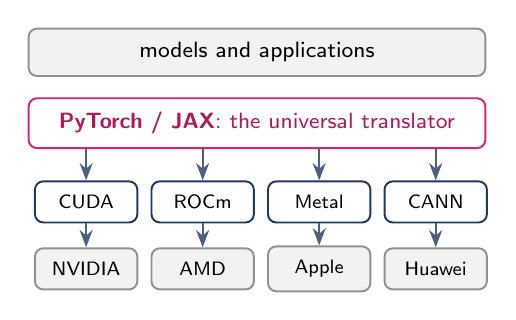
\begin{tikzpicture}[x=1cm,y=1cm]
  \node[softbox,minimum width=5.8cm] (apps) at (2.9,3.0) {models and applications};
  \node[hot,minimum width=5.8cm] (pt) at (2.9,2.1) {\textbf{PyTorch / JAX}: the universal translator};
  \foreach \i/\p/\h in {0/CUDA/NVIDIA, 1/ROCm/AMD, 2/Metal/Apple, 3/CANN/Huawei}{
    \node[box,minimum width=1.3cm,font=\scriptsize] (p\i) at (0.73+1.48*\i,1.1) {\p};
    \node[softbox,minimum width=1.3cm,font=\scriptsize] (h\i) at (0.73+1.48*\i,0.25) {\h};
    \draw[arr] (pt.south -| p\i.north) -- (p\i.north);
    \draw[arr] (p\i) -- (h\i);}
\end{tikzpicture}
\vspace{0.15cm}

{\scriptsize The lock-in of CUDA weakens as backends for other hardware mature.}
\end{column}
\end{columns}
\source{DeepSeek-AI (2024), DeepSeek-V3 technical report; Reuters reporting on the Shenzhen EUV prototype (late 2025).}
\end{frame}
% NOTES: Export controls oscillate between "deny" and "retain";
% Beijing also uses access as leverage (H200 episode, early 2026).

% ============================================================
% 10. TWO BETS: MINDS AND BODIES
% ============================================================
\begin{frame}{Two bets? Minds and bodies}
\begin{center}
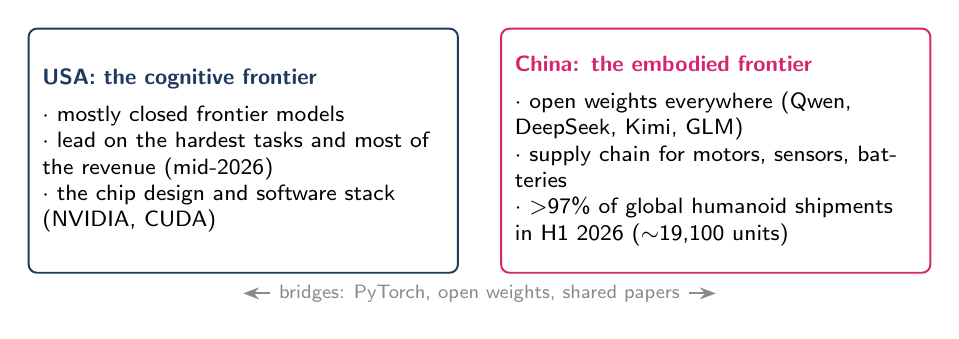
\begin{tikzpicture}
  \node[box,text width=5.1cm,align=left,minimum height=3.1cm,anchor=north] (us) at (-3.0,0) {
    {\bfseries\color{navy} USA: the cognitive frontier}\\[4pt]
    $\cdot$ mostly closed frontier models\\
    $\cdot$ lead on the hardest tasks and most of the revenue (mid-2026)\\
    $\cdot$ the chip design and software stack (NVIDIA, CUDA)};
  \node[hot,text=black,text width=5.1cm,align=left,minimum height=3.1cm,anchor=north] (cn) at (3.0,0) {
    {\bfseries\color{magenta} China: the embodied frontier}\\[4pt]
    $\cdot$ open weights everywhere (Qwen, DeepSeek, Kimi, GLM)\\
    $\cdot$ supply chain for motors, sensors, batteries\\
    $\cdot$ $>$97\% of global humanoid shipments in H1 2026 ($\sim$19{,}100 units)};
  \draw[{Stealth[length=2mm]}-{Stealth[length=2mm]},line width=0.8pt,midgray]
     ($(us.south)+(0,-0.25)$) -- node[fill=white,font=\scriptsize,text=midgray]{bridges: PyTorch, open weights, shared papers} ($(cn.south)+(0,-0.25)$);
\end{tikzpicture}
\end{center}
\vspace{0.1cm}
\small A hypothesis, not a law: shipments are not value, and both sides compete on both fronts.
But if intelligence leaves the screen, \alert{who builds the bodies} may matter as much as who trains the minds.
\source{Smart Analytics Global, humanoid robot shipments report (Aug 2026), via Bloomberg/TechRepublic.}
\end{frame}
% NOTES: AgiBot ~8,400 and Unitree ~5,900 units in H1 2026, far above
% Tesla, Figure, Agility. Commercially productive deployments still small.

% ============================================================
% 11. SCENARIOS
% ============================================================
\begin{frame}{Four possible futures (not mutually exclusive)}
\begin{center}
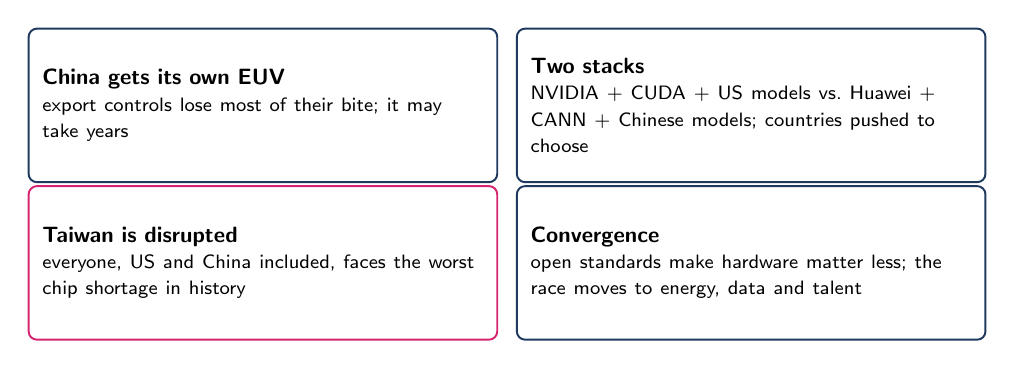
\begin{tikzpicture}
  \tikzset{scen/.style={box,text width=5.6cm,align=left,minimum height=1.95cm}}
  \node[scen] (s1) at (-3.1,1.0) {\textbf{China gets its own EUV}\\{\scriptsize export controls lose most of their bite; it may take years}};
  \node[scen] (s2) at (3.1,1.0) {\textbf{Two stacks}\\{\scriptsize NVIDIA + CUDA + US models vs.\ Huawei + CANN + Chinese models; countries pushed to choose}};
  \node[scen,draw=magenta] (s3) at (-3.1,-1.0) {\textbf{Taiwan is disrupted}\\{\scriptsize everyone, US and China included, faces the worst chip shortage in history}};
  \node[scen] (s4) at (3.1,-1.0) {\textbf{Convergence}\\{\scriptsize open standards make hardware matter less; the race moves to energy, data and talent}};
\end{tikzpicture}
\end{center}
\vspace{0.1cm}
\small All four depend on political decisions as much as on technical progress.
\end{frame}
% NOTES: Keep it to 45 seconds. The fourth one is the hopeful one for us.

% ============================================================
% 12. WHAT ABOUT US?
% ============================================================
\begin{frame}{And from the South?}
We don't make the chips, but we are not spectators.
\begin{itemize}
  \item \textbf{Open weights} let us run, adapt and audit models on our own soil, with our own data.
  \item \textbf{Energy and minerals} are part of the AI chain, and Chile has both.
  \item \textbf{Verification and data}: benchmarks, languages and problems that are ours.
  \item \textbf{Safety} is a shared job: AI and security communities must work together.
\end{itemize}
\vfill
\begin{center}
{\large\color{navy}\bfseries Thank you!}\\[2pt]

\includegraphics[height=0.75cm]{logos/dcc.pdf}\hspace{0.8cm}

\includegraphics[height=0.5cm]{logos/cenia.png}\hspace{0.8cm}

\includegraphics[height=0.55cm]{logos/idia.png}
\end{center}
\end{frame}
% NOTES: End on the message: the frontier is not only in San Francisco
% and Shenzhen; the questions of what to build, and for whom, are ours too.

\end{document}
